% !TEX TS-program = XeLaTeX
% use the following command:
% all document files must be coded in UTF-8
\documentclass[spanish]{textolivre}
% build HTML with: make4ht -e build.lua -c textolivre.cfg -x -u article "fn-in,svg,pic-align"

\journalname{Texto Livre}
\thevolume{15}
%\thenumber{1} % old template
\theyear{2022}
\receiveddate{\DTMdisplaydate{2021}{12}{3}{-1}} % YYYY MM DD
\accepteddate{\DTMdisplaydate{2022}{1}{19}{-1}}
\publisheddate{\DTMdisplaydate{2022}{4}{28}{-1}}
\corrauthor{Angela María Lopera Molano}
\articledoi{10.35699/1983-3652.2022.37365}
%\articleid{NNNN} % if the article ID is not the last 5 numbers of its DOI, provide it using \articleid{} commmand 
% list of available sesscions in the journal: articles, dossier, reports, essays, reviews, interviews, editorial
\articlesessionname{articles}
\runningauthor{Lopera Molano} 
%\editorname{Leonardo Araújo} % old template
\sectioneditorname{Daniervelin Pereira}
\layouteditorname{Carolina Garcia}

\title{Apropiación social de las TIC y asociaciones agrícolas del sector rural: revisión sistemática de la literatura 2010-2020}
\othertitle{Apropriação social das TIC e associações agrícolas no setor rural: revisão sistemática da literatura 2010-2020}
\othertitle{Social appropriation of ICT and agricultural associations in the rural sector: systematic literature review 2010-2020}
% if there is a third language title, add here:
%\othertitle{Artikelvorlage zur Einreichung beim Texto Livre Journal}

\author[1,2]{Angela María Lopera Molano \orcid{0000-0002-3797-7996} \thanks{Email: \url{angela.lopera@unibague.edu.co}}}
\affil[1]{Universidad de La Sabana, Facultad de Comunicación, Doctorado en Comunicación, Cundinamarca, Colombia.}
\affil[2]{Universidad de Ibagué, Facultad de Humanidades, Artes y Ciencias sociales, Programa de Comunicación social y Jornalismo, Ibagué, Tolima, Colombia.}


\addbibresource{article.bib}
% use biber instead of bibtex
% $ biber article

% used to create dummy text for the template file
\definecolor{dark-gray}{gray}{0.35} % color used to display dummy texts
\usepackage{lipsum}
\SetLipsumParListSurrounders{\colorlet{oldcolor}{.}\color{dark-gray}}{\color{oldcolor}}

% used here only to provide the XeLaTeX and BibTeX logos
\usepackage{hologo}

% if you use multirows in a table, include the multirow package
\usepackage{multirow}

% provides sidewaysfigure environment
\usepackage{rotating}

% CUSTOM EPIGRAPH - BEGIN 
%%% https://tex.stackexchange.com/questions/193178/specific-epigraph-style
\usepackage{epigraph}
\renewcommand\textflush{flushright}
\makeatletter
\newlength\epitextskip
\pretocmd{\@epitext}{\em}{}{}
\apptocmd{\@epitext}{\em}{}{}
\patchcmd{\epigraph}{\@epitext{#1}\\}{\@epitext{#1}\\[\epitextskip]}{}{}
\makeatother
\setlength\epigraphrule{0pt}
\setlength\epitextskip{0.5ex}
\setlength\epigraphwidth{.7\textwidth}
% CUSTOM EPIGRAPH - END

% LANGUAGE - BEGIN
% ARABIC
% for languages that use special fonts, you must provide the typeface that will be used
% \setotherlanguage{arabic}
% \newfontfamily\arabicfont[Script=Arabic]{Amiri}
% \newfontfamily\arabicfontsf[Script=Arabic]{Amiri}
% \newfontfamily\arabicfonttt[Script=Arabic]{Amiri}
%
% in the article, to add arabic text use: \textlang{arabic}{ ... }
%
% RUSSIAN
% for russian text we also need to define fonts with support for Cyrillic script
% \usepackage{fontspec}
% \setotherlanguage{russian}
% \newfontfamily\cyrillicfont{Times New Roman}
% \newfontfamily\cyrillicfontsf{Times New Roman}[Script=Cyrillic]
% \newfontfamily\cyrillicfonttt{Times New Roman}[Script=Cyrillic]
%
% in the text use \begin{russian} ... \end{russian}
% LANGUAGE - END

% EMOJIS - BEGIN
% to use emoticons in your manuscript
% https://stackoverflow.com/questions/190145/how-to-insert-emoticons-in-latex/57076064
% using font Symbola, which has full support
% the font may be downloaded at:
% https://dn-works.com/ufas/
% add to preamble:
% \newfontfamily\Symbola{Symbola}
% in the text use:
% {\Symbola }
% EMOJIS - END

% LABEL REFERENCE TO DESCRIPTIVE LIST - BEGIN
% reference itens in a descriptive list using their labels instead of numbers
% insert the code below in the preambule:
%\makeatletter
%\let\orgdescriptionlabel\descriptionlabel
%\renewcommand*{\descriptionlabel}[1]{%
%  \let\orglabel\label
%  \let\label\@gobble
%  \phantomsection
%  \edef\@currentlabel{#1\unskip}%
%  \let\label\orglabel
%  \orgdescriptionlabel{#1}%
%}
%\makeatother
%
% in your document, use as illustraded here:
%\begin{description}
%  \item[first\label{itm1}] this is only an example;
%  % ...  add more items
%\end{description}
% LABEL REFERENCE TO DESCRIPTIVE LIST - END


% add line numbers for submission
%\usepackage{lineno}
%\linenumbers

\begin{document}
\maketitle

\begin{polyabstract}
\begin{abstract}
La apropiación social de las TIC en contextos rurales es un desafío para los gobiernos y los agricultores, que requieren de las TIC para fortalecer los procesos de producción y comercialización, a través de proyectos para la inclusión y la alfabetización digital. El propósito de este artículo es analizar cómo se ha estudiado este fenómeno, desde qué enfoques o perspectivas teóricas y cuáles son los abordajes necesarios a futuro para lograr la apropiación social de las TIC en el sector agrícola. Una revisión sistemática de la literatura identificó cuatro líneas de investigación, desde 2010 a 2020. La tendencia principal es hacia el estudio de los usos y la adopción de las TIC, a partir de la identificación de variables cuantitativas de uso y no uso; también aparecen investigaciones centradas en los procesos de apropiación social, no solo para la agricultura, sino para la vida cotidiana de las comunidades, que es donde debe iniciar la alfabetización digital. Se pudo concluir que la línea de investigación sobre apropiación social tiene un componente conceptual y metodológico que la diferencia de los estudios de usos y adopción de las TIC, porque se enfoca en el reconocimiento autónomo que hacen los agricultores sobre los beneficios o debilidades del uso de las TIC; además, hay una desconexión entre la identificación de los usos y cómo éstos pueden contribuir a los procesos de apropiación de las TIC en el sector agrícola, lo que implica un acercamiento metodológico cualitativo y no solo la medición cuantitativa.

\keywords{Apropiación tecnológica \sep Tecnologías de la Información y la Comunicación (TIC) \sep Desarrollo rural \sep Agricultura}
\end{abstract}

\begin{portuguese}
\begin{abstract}
A apropriação social das TIC em contextos rurais é um desafio para governos e agricultores, que as requerem para reforçar os processos de produção e comercialização, através de projetos de inclusão e letramento digital. O objetivo deste artigo é analisar como este fenômeno foi estudado, a partir de quais abordagens ou perspectivas teóricas e quais são as abordagens futuras necessárias para conseguir a apropriação social das TIC no setor agrícola. Uma revisão sistemática da literatura identificou quatro linhas de pesquisa, de 2010 a 2020. A principal tendência se refere ao estudo dos usos à adoção das TIC, com base na identificação de variáveis quantitativas de uso e não uso; há também uma linha de pesquisa centrada nos processos de apropriação social, não só para a agricultura, mas também para a vida quotidiana das comunidades, que é onde o letramento digital deve começar. Foi possível concluir que a linha de pesquisa sobre apropriação social tem um componente conceitual e metodológico que a diferencia dos estudos de utilização e adoção das TIC, porque se centra no reconhecimento autônomo pelos agricultores dos benefícios ou desvantagens da utilização das TIC; além disso, existe uma desconexão entre a identificação dos usos e a forma como esses podem contribuir para os processos de apropriação das TIC no setor agrícola, o que implica uma abordagem metodológica qualitativa e não apenas quantitativa. 

\keywords{Apropriação tecnológica \sep Tecnologias de Informação e Comunicação (TIC) \sep Desenvolvimento rural \sep Agricultura}
\end{abstract}
\end{portuguese}

\begin{english}
\begin{abstract}
Social appropriation of ICTs in rural contexts is a challenge for governments and farmers, who require ICTs to strengthen production and marketing processes through projects for inclusion and digital literacy. The purpose of this article is to analyze how this phenomenon has been studied, from what approaches or theoretical perspectives and what future approaches are needed to achieve social appropriation of ICTs in the agricultural sector. A systematic review of the literature identified four lines of research, from 2010 to 2020. The main trend is toward the study of the uses and adoption of ICTs, based on the identification of quantitative variables of use and non-use; there is also research focused on the processes of social appropriation, not only for agriculture, but also for the daily life of communities, which is where digital literacy should begin. It was possible to conclude that the line of research on social appropriation has a conceptual and methodological component that differentiates it from studies of ICT uses and adoption, because it focuses on the autonomous recognition by farmers of the benefits or weaknesses of ICT use; in addition, there is a disconnection between the identification of uses and how these can contribute to the processes of appropriation of ICTs in the agricultural sector, which imply a qualitative methodological approach and not only quantitative measurement.

\keywords{Technological appropriation \sep Information and Communication Technologies (ICT) \sep Rural development \sep Agriculture}
\end{abstract}
\end{english}
% if there is another abstract, insert it here using the same scheme
\end{polyabstract}

\section{Introducción}\label{sec-intro}

Las Tecnologías de la Información y la Comunicación, TIC, son herramientas digitales de uso masivo. Son también definidas como un medio de comunicación que contribuye para la transformación de problemáticas sociales. Por lo tanto, las TIC son herramientas (dispositivos, artefactos) culturales \cite{santini_uso_2017,andres_aproximacion_2014,benitz_larghi_apropiacion_2016,paulhiac_perez_uso_2019, acosta_nates_culturas_2014,barbosa_trigos_propuesta_2016}. Esto quiere decir que las TIC se modifican y modifican “los modos de comunicar e informar […], debido a las configuraciones particulares de los dispositivos mediáticos” \cite[p.~18]{andres_aproximacion_2014}. Por lo tanto, las TIC interactúan con los sujetos en sus respectivos contextos. No basta con hablar de infraestructura, porque al ser las TIC medios de comunicación, se incluyen también los contenidos, destrezas, conocimientos y capacidades involucradas de los sujetos en su relación con éstas \cite{bossio_desarrollo_2005}. 

Las TIC son medios para alcanzar objetivos de desarrollo de las comunidades \cite{paulhiac_perez_uso_2019,duarte_metodologipara_2014,castro_hidalgo_impacto_2014,barbosa_trigos_propuesta_2016}, entendiendo estas tecnologías como posibilitadores o facilitadores de procesos en contextos situados. En tal sentido, las TIC también favorecen la producción de conocimiento, son “herramientas para la gestión de iniciativas” \cite[p.~40]{duarte_metodologipara_2014}; posibilitan “el trabajo colaborativo, el aprendizaje ubicuo, las redes sociales digitales” \cite[p.~4-5]{santini_uso_2017} o de gestión de conocimiento \cite{santini_uso_2018}. Lo anterior depende del contexto cultural, los actores, los espacios y tiempos sociales, los objetivos, las conductas, valoraciones y expectativas \cite{sanchez_davila_nuevas_2018} que se generan al interactuar con las TIC. 

En las dos últimas décadas se ha visto una expansión de las tecnologías digitales para la información y la innovación, convirtiéndose en un factor determinante para mejorar la productividad económica en el sector agrícola, lograr el acceso de los pequeños agricultores al mercado y reducir la pobreza. Pero las zonas rurales aún tienen una infraestructura deficiente y una baja capacidad de servicios de información, además de “las limitaciones logísticas, como las instalaciones de transporte y las carreteras de acceso a las comunidades y mercados agrícolas y desde ellos […]” \cite[p.~47]{owusu_smallholder_2017}. Los agricultores se encuentran con la barrera del acceso material a las tecnologías y los altos costos del servicio. Además de lo anterior, existen limitantes para la adopción de las TIC como el pobre entendimiento de su valor, impedimentos personales (como habilidades y alfabetización) \cite{matsenjwa_pro-poor_2019}, nivel de uso muy bajo y capacidades desarrolladas \cite{vong_empowering_2019}. 

Este texto se enfoca en los estudios sobre los procesos para la apropiación social de las TIC como una fase esencial para la transformación de las comunidades rurales del sector agrícola y para aportar al desarrollo rural. De allí que un escenario ideal de estudio no solo implica identificar los usos de las TIC en las asociaciones agrícolas, sino su conexión con los procesos contextualizados (particularidades geográficas, culturales y sociales) que permitan desarrollar habilidades digitales para su posterior apropiación social.

 Una revisión sistemática de la literatura permite responder tres preguntas enfocadas en las afirmaciones anteriores:

\begin{enumerate}
    \item ¿Cuáles son los principales enfoques, perspectivas teóricas y conclusiones que surgen de las investigaciones sobre la apropiación social de las TIC en comunidades rurales agrícolas?
    \item 	¿Cuáles son las conexiones que se establecen entre los usos de las TIC y los procesos de apropiación social que se han dado en el contexto agrícola rural?
    \item ¿Cuáles son los posibles abordajes para las investigaciones futuras sobre el tema, que pueden contribuir a la implementación de procesos para la apropiación social de las TIC en contextos agrícolas rurales?
\end{enumerate}

Al responder estas preguntas se pueden identificar las principales tendencias en investigación reciente sobre el tema en cuestión, así como las conclusiones para consolidar la línea de trabajo sobre la apropiación social de las TIC en el sector agrícola. También, es posible poner en diálogo las recomendaciones de los investigadores en términos de la apropiación social, con los esfuerzos constantes de los gobiernos por brindar conectividad al sector rural. 

Lo anterior cobra relevancia en la medida que se entienda que las TIC son herramientas posibilitadoras y no la solución a los problemas del sector agrícola. La identificación de las trayectorias de uso, tanto de los individuos como de las organizaciones o asociaciones, son esenciales para pensar y proponer procesos de formación para la apropiación social de las TIC \cite{crovi_drueta_dimension_2008}, para el beneficio de los actores centrales que son los campesinos de las asociaciones agrícolas; así sea solamente un eslabón del proceso que podrá conectar, a futuro, con los intereses productivos de los planes TIC y los planes para el sector agropecuario.

De igual manera, desde revisiones previas de la literatura se ha comenzado a delimitar una línea de investigación sobre la apropiación de las TIC en el sector agrícola que, como se verá más adelante, se encuentra fragmentada en dos aspectos: 1) la fragmentación de la discusión sobre el uso y la apropiación de las TIC, ya que se ha trabajado desde disciplinas agregadas y no desde enfoques transdisciplinares y 2) las investigaciones separan los usos y las apropiaciones del sector agrícola de otros espacios de la cotidianidad de los campesinos. Nuevas contribuciones a esta línea de investigación, como el caso de esta revisión sistemática de la literatura, no solo pretenden desarrollarla sino fortalecerla, al tratar de superar las fragmentaciones señaladas.

Los apartados que siguen se organizan de la siguiente manera. En la segunda sección se presenta la aproximación teórica que sustenta la investigación. En la tercera sección se aborda la metodología y se describe detalladamente el proceso desarrollado, así como los instrumentos utilizados. En la cuarta sección se presentan los principales hallazgos del estudio y las líneas de investigación que resultaron de la interpretación de los estudios previos. Finalmente, en la quinta y sexta secciones se presentan la discusión y las conclusiones de la investigación.

\section{La apropiación social de las TIC en sectores agrícolas rurales}

Investigaciones anteriores han demostrado cómo las TIC generan cambios socioeconómicos en las comunidades campesinas, pero solo en la medida que sus beneficios son aprovechados por quienes las utilizan \cite{sanchez_davila_nuevas_2018,zapata_-_cardenas_ruralidad_2015,castro_hidalgo_impacto_2014,barbosa_trigos_propuesta_2016,santini_uso_2017}. Lo anterior implica que las TIC por sí solas no generan los cambios, sino que interactúan con las personas y se resignifican desde allí.

La perspectiva social o sociocultural \cite{sandoval_algunos_2017} del estudio de las tecnologías se interesa por los sentidos que éstas adquieren en la vida cotidiana y dialoga de manera crítica con perspectivas deterministas, fundadas en una racionalidad instrumental \cite{lopez_apropiarse_2017}.

La brecha, la desigualdad y la inclusión digital; infraestructura, acceso, conectividad, y las denominadas Tecnologías de la Información y la Comunicación, TIC, articulan un escenario de preocupaciones compartidas sobre nuevas desigualdades sociales que se evidencian en la era digital \cite{rivoir_reflexiones_2017}, a raíz de la rápida expansión de Internet durante la década de los noventa y los acelerados cambios posteriores en las tecnologías digitales \cite{lago_martinez_teori_2017}. Este escenario hace que emerjan conceptos como el de apropiación o apropiación de tecnologías, pero también que se prioricen estudios de grupos sociales en situación de desigualdad, con la salvedad que la brecha digital no se supera solamente con acceso, uso y habilidades digitales \cite{lago_martinez_teori_2017}.

Este contexto particular de surgimiento de la categoría de apropiación para el estudio de las tecnologías digitales lo marcan aspectos transversales tales como: 1) el campo de estudio interdisciplinar, porque se trata de un problema complejo; 2) el desarrollo tecnológico acelerado implica que las TIC están en movimiento constante, que no se refieren a un solo artefacto, sino a muchos y en constante cambio; 3) los procesos de desarrollo y cambio social que también interfieren en esta mirada, por ejemplo, las TIC para el desarrollo; 4) la transformación hacia comunidades virtuales productoras de contenidos y no solo consumidoras; 5) la importancia de la infraestructura y la conectividad, así como los usos y las prácticas de apropiación \cite{rivoir_reflexiones_2017}. 

Lo anterior plantea un desafío para el desarrollo rural \cite{alavion_rural_2020}, porque contribuye a cerrar la brecha digital y promueve la equidad urbano-rural \cite{ye_citizen-led_2021}. Sin embargo, los esfuerzos dependen de la manera en la que se involucra a la comunidad en los procesos para adoptar nuevas tecnologías, porque se requiere de su participación y empoderamiento \cite{matsenjwa_pro-poor_2019}. 

\section{Metodología}\label{sec-modelo}

La investigación documental como método científico de estudio, desde el enfoque cualitativo, genera un acercamiento crítico a un grupo amplio de investigaciones sobre una problemática específica, con el fin de identificar posturas teóricas y metodológicas \cite{gomez_vargas_estado_2015} y permite “localizar, procesar y reconstruir información relevante para un tema en tres sentidos: de acuerdo a su fuente, al proceso de análisis implicado y al resultado esperado” \cite[p.~3]{izaguirre_remon_revision_nodate}.

La revisión documental identifica: 1) qué se ha estudiado previamente sobre el tema, lo cual permite esclarecer los enfoques investigativos, 2) el contexto conceptual del problema de investigación, así como los métodos usados \cite{izaguirre_remon_revision_nodate}, y 3) extrae las conclusiones relevantes, a través de la interpretación sistemática de los estudios, para proponer abordajes futuros sobre el tema. 

Este proceso se caracteriza por ser sistemático en la medida en que se desarrolla de forma minuciosa y rigurosa, a partir de instrumentos que reseñan categorías centrales de los textos y acordes con el propósito del estudio y problemática expuesta.

\subsection{Descripción del proceso metodológico}

La revisión sistemática de la literatura se concentró en identificar todos aquellos acercamientos que se han realizado a partir de los usos y las apropiaciones de las TIC en contextos rurales de producción agrícola. La primera búsqueda se realizó en la base de datos de SCOPUS en un periodo de tiempo de cinco años, desde 2016 a 2020, a partir de las siguientes palabras claves en español y en inglés: ICT + RURAL, ICT + RURAL + ADOPTION, ICT + RURAL + INCLUSION, ICT + RURAL + DEVELOPMENT. En esta búsqueda se filtraron 37 artículos relacionados con el tema.

Sin embargo, se identificaron dos limitaciones, la primera, que los artículos en inglés no usan el concepto de \textit{apropiación}, sino que se utiliza como equivalente el concepto de \textit{adopción}. No obstante, como en español se diferencian los dos términos tanto conceptualmente como en la práctica, era necesario ampliar la búsqueda. La segunda limitación es que la mayoría de los estudios encontrados eran asiáticos y africanos, lo cual es positivo, pero no permite conocer el panorama más cercano de lo que sucede en América Latina, con respecto al tema de estudio; de este último continente solo se encontraron cuatro investigaciones Por las razones expuestas previamente se decidió ampliar la búsqueda a WOS y Google Scholar, además, ampliar el tiempo desde 2010 hasta 2020. En esta nueva búsqueda se filtraron 26 investigaciones más que se relacionan directamente con el tema, para un total de 63 estudios revisados. 

En una matriz construida en Excel se reseñaron todas las investigaciones y se identificaron aspectos puntuales que permitían abordar las preguntas de investigación, tales como: país del estudio, disciplina o disciplinas desde las que se aborda el estudio, propósito de la investigación, marco teórico, metodología, conclusiones, recomendaciones, enfoque de la investigación y, finalmente, observaciones de cada texto. En el caso específico del marco teórico, se identificó que las investigaciones acuden a términos tales como: acceso, uso, adopción y apropiación. 

Toda esta información obtenida se revisó en un segundo proceso de lectura de los textos y se procedió a clasificar los documentos por cada una de las categorías de la primera matriz para identificar las mayores coincidencias, por ejemplo: los países con los enfoques; las metodologías con los enfoques de las investigaciones; las metodologías con los propósitos de las investigaciones; las disciplinas con los enfoques metodológicos; el marco teórico con los enfoques y las metodologías. Este último cruce de información fue central para determinar el problema de estudio de cada una de las investigaciones y de qué manera se propone abordarlo tanto teórica como metodológicamente por parte de los autores. Dicha delimitación del problema de estudio señaló afinidades y diferencias, que determinaron las líneas de investigación propuestas para esta revisión de la literatura. 

De esta manera, se procedió, en una segunda matriz de Excel, a organizar los estudios en las siguientes líneas de investigación: 1) Usos e impactos del uso de las TIC en contextos agrícolas rurales; 2) Adopción de las TIC en contextos rurales de producción agrícola; 3) Apropiación social de las TIC en contextos rurales de producción agrícola; y 4) Modelos para la apropiación social.

\section{Resultados}\label{sec-organizacao}

Los autores de las 63 investigaciones provienen de disciplinas y campos de estudio diferentes, por ejemplo, de la economía, administración, geografía, ciencias agrícolas, estudios del desarrollo, negocios (agronegocios), estudios rurales, ingeniería, tecnología y desde la comunicación, que se encuentran en mayor medida en los estudios latinoamericanos. Esto permite afirmar, como lo dicen los mismos autores, que este tema se ha abordado de manera interdisciplinar, desde enfoques tanto cuantitativos como cualitativos. Lo anterior significa que se trata de un problema histórico y complejo que no puede ser observado o estudiado desde la fragmentación disciplinar. Lo anterior repercute en los abordajes teóricos, como se detalla más adelante. 

Los países en los que se desarrollan las investigaciones pertenecen, en su mayoría, al continente asiático, africano y latinoamericano (\Cref{fig1}). Todos tienen en común situaciones que afectan al contexto rural, una aproximación a las TIC como herramientas que posibilitan un cambio para la economía del sector agrícola y también visiones desde el desarrollo rural o las TIC para el desarrollo rural; aspectos que ampliamos a continuación. 

\begin{figure}[htbp]
\centering
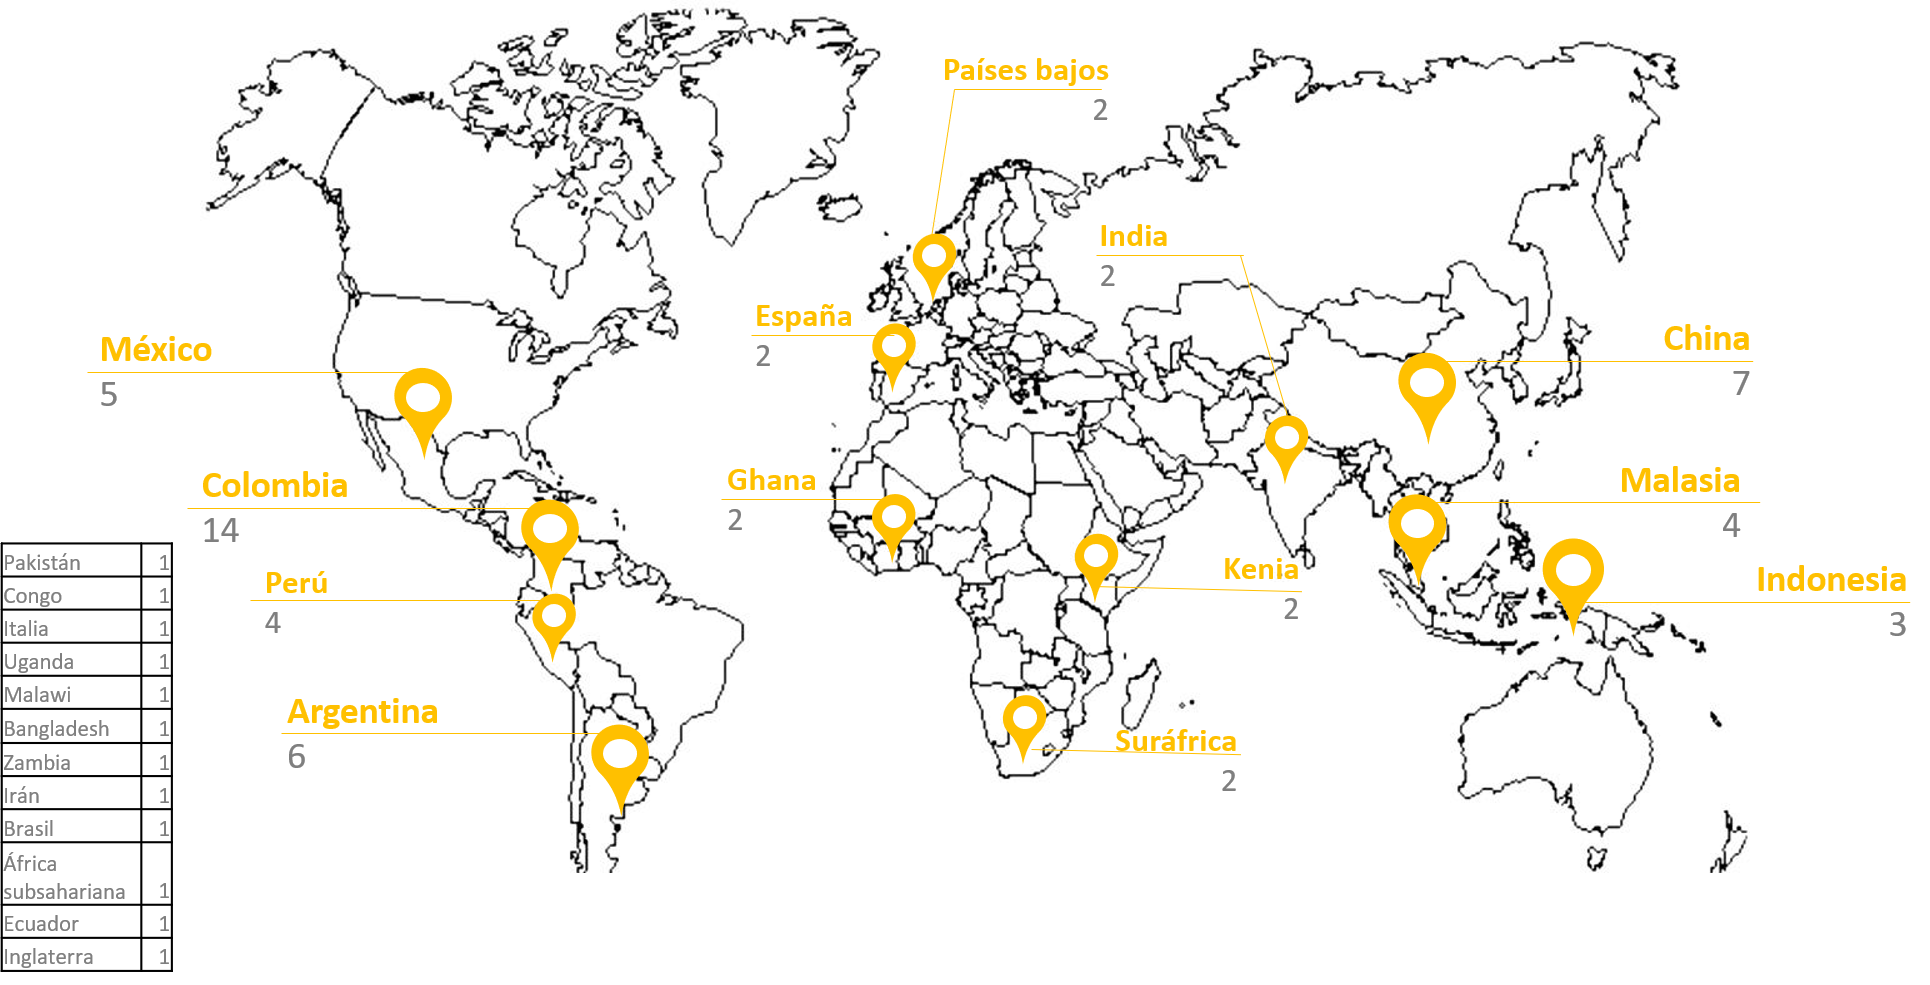
\includegraphics[width=0.85\textwidth]{fig1.png}
\caption{Países de estudio de los usos y apropiaciones de las TIC.}
\label{fig1}
\source{Elaboración propia.}
\end{figure}

Las investigaciones presentan un panorama del contexto rural que se comparte en la mayoría de los países. En primer lugar, que la agricultura es un sector central en la economía, pero que las zonas rurales tienen una infraestructura deficiente y baja capacidad de servicios de información. En segundo lugar, las investigaciones señalan que en las dos últimas décadas se ha visto una expansión de las tecnologías digitales para la información y la innovación, por lo tanto, el acceso a la información es un factor determinante para mejorar la productividad económica en el sector agrícola. En tercer lugar, y ya de manera más puntual, ciertas investigaciones tienen presente el debate sobre el desarrollo, al afirmar que existe una línea de investigación enfocada en fomentar el desarrollo a través de las TIC \cite{ye_citizen-led_2021}. Los diferentes autores consideran que la automatización de los procesos a través de las TIC ayudará a reducir la pobreza en los países en desarrollo, sin embargo, los proyectos que se plantean no alcanzan sus objetivos \cite{perez-estebanez_technological_2018} porque la tecnología es solo un aspecto de otros muchos que se deben atender en los países pobres para lograr ese impacto económico \cite{min_does_2020}. Otra perspectiva, que se considera una disciplina agregada, son las TIC para el desarrollo (TIC4D por sus siglas en inglés), que nace en los años 90 \cite{mariscal_aviles_informational_2016}. Desde este enfoque, la apropiación de las TIC solo es posible en los procesos que nacen de las mismas comunidades. 

A continuación, se abordan las cuatro líneas de investigación identificadas en la revisión sistemática de la literatura.

\subsection{Usos e impactos del uso de las TIC en contextos rurales }

La primera línea de investigación la componen la mayoría de los trabajos, los cuales estudian los usos e impactos del uso de las TIC en contextos agrícolas rurales (\Cref{fig2}). Hay 26 investigaciones que se relacionan con este primer acercamiento, de 17 países diferentes, especialmente de China y Perú.

\begin{figure}[htbp]
\centering
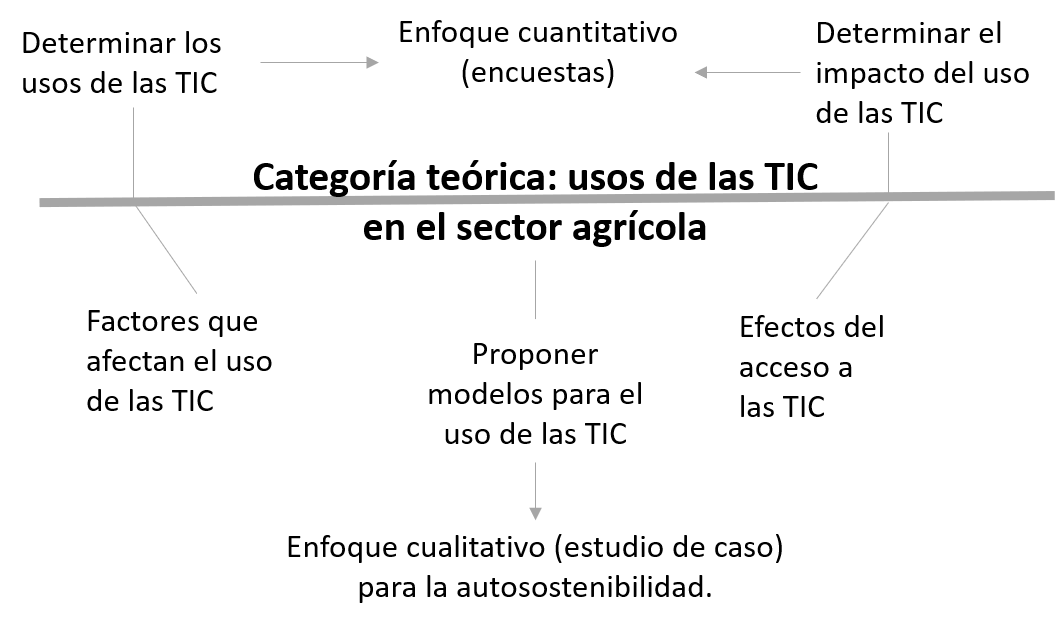
\includegraphics[width=0.85\textwidth]{fig2.png}
\caption{Primera línea de investigación.}
\label{fig2}
\source{Elaboración propia.}
\end{figure}

Desde estos estudios, las TIC son un posibilitador e innovador social para las áreas rurales, pueden mejorar los servicios de salud, sociales, educación, energía, transporte y comercio minorista, haciéndolos más sostenibles mediante el despliegue de herramientas TIC y a través de acciones y proyectos comunitarios y empresariales \cite{ievoli_information_2019}. 

Por lo tanto, según estas investigaciones, es determinante conocer los factores que posibilitan el uso de las TIC, que son: el nivel educativo, las habilidades para el uso del teléfono, tener un teléfono durante más tiempo y el número de teléfonos en la familia \cite{khan_farmers_2020}. En el uso activo de las TIC intervienen factores como las características de los hogares y las familias, lo que significa que poseer la tecnología no garantiza su uso, es más importante usarla activamente \cite{sheng_influence_2020}. Pero también incide el género, tamaño de la granja y el trabajo fuera de la granja \cite{ma_smartphone_2020}. Finalmente, el uso de las TIC en la agricultura está directamente relacionado con el adecuado nivel de capacitación en TIC \cite{perez-estebanez_technological_2018}. Las subcategorías encontradas en esta línea se enfocan en el uso de las TIC o la innovación social, el empoderamiento y la relación con la vida cotidiana (\Cref{fig3}). 

\begin{figure}[htbp]
\centering
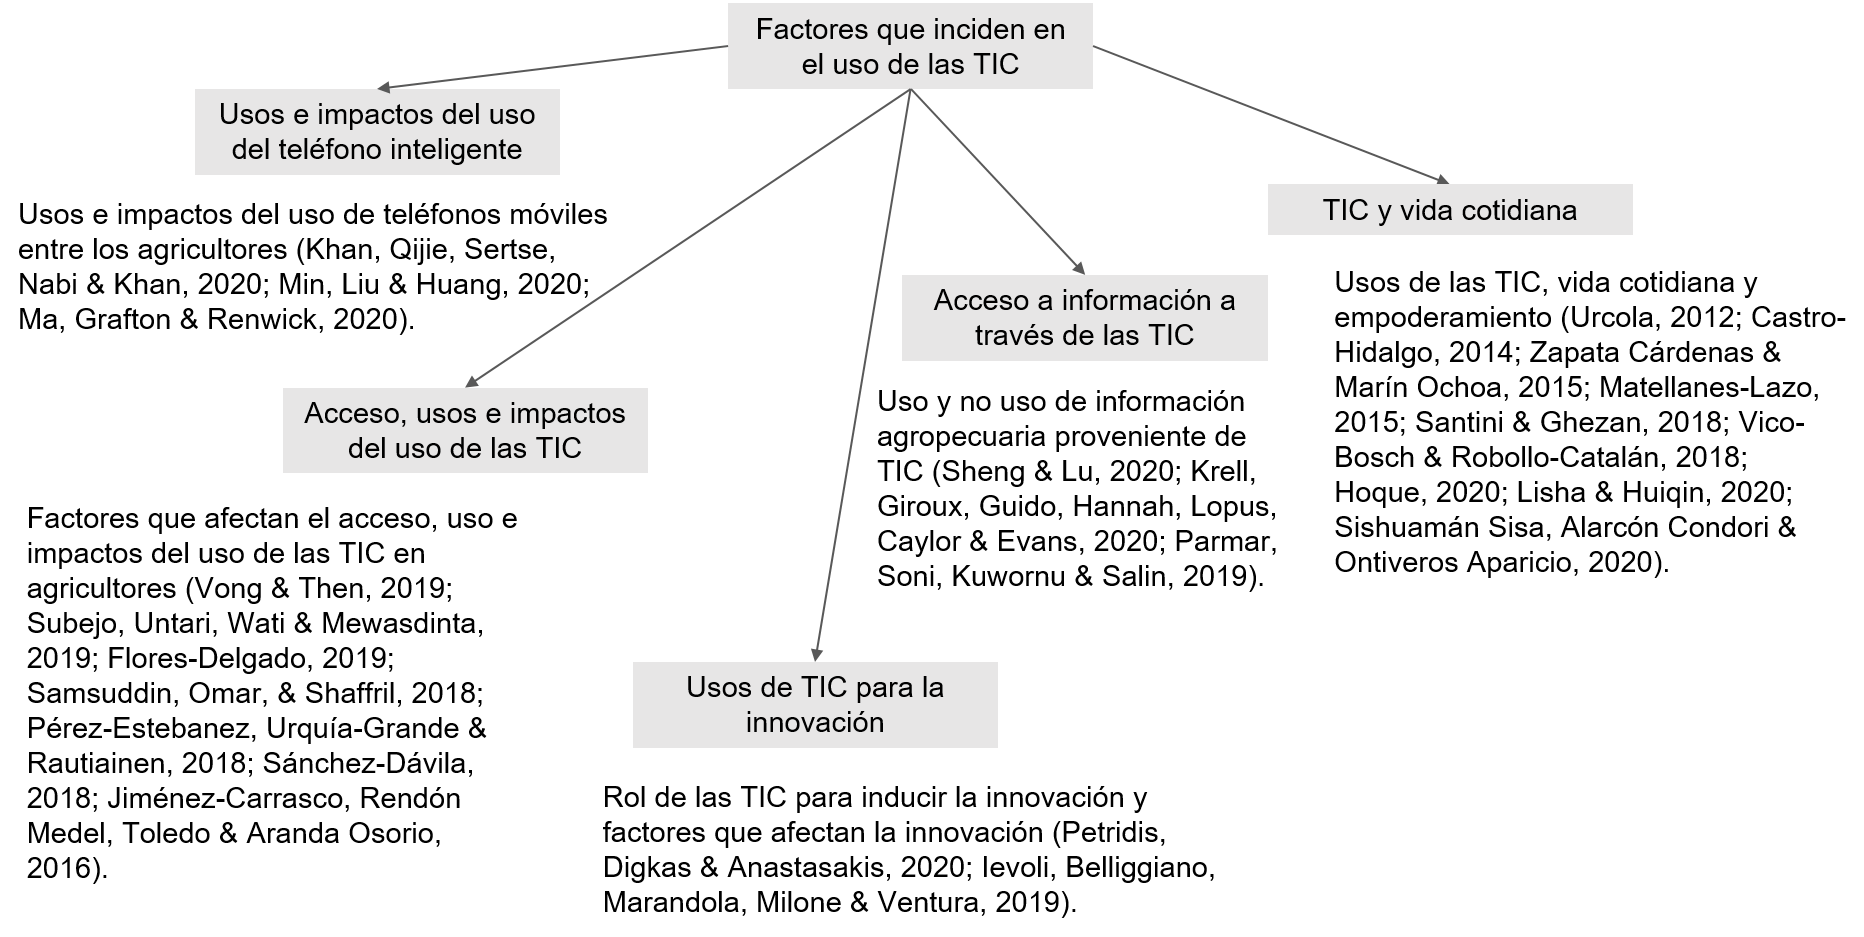
\includegraphics[width=0.85\textwidth]{fig3.png}
\caption{Los diferentes usos de las TIC.}
\label{fig3}
\source{Elaboración propia con base en \textcite{khan_farmers_2020,min_does_2020,ma_smartphone_2020,vong_empowering_2019,subejo_modernization_2019,flores_delgado_campesino_2019,samsuddin_youth_2018,perez-estebanez_technological_2018,sanchez_davila_nuevas_2018,jimenez_carrasco_tecnologias_2016,sheng_influence_2020,krell_smallholder_2021,parmar_evaluating_2019,urcola_articulacion_2012,castro_hidalgo_impacto_2014,zapata_-_cardenas_ruralidad_2015,matellanes-lazo_uso_2015,santini_uso_2018,vico-bosch_incidencia_2018,hoque_impact_2020,ye_citizen-led_2021,susihuaman_sisa_tecnologias_2020,petridis_factors_2020,ievoli_information_2019}.}
\end{figure}

Algunas de las recomendaciones que manifiestan los mismos autores de los estudios son: la necesidad de una educación para desarrollar habilidades digitales que no tienen los campesinos \cite{khan_farmers_2020,vong_empowering_2019}; el fortalecimiento de la capacitación en tecnología, lo que significa aumentar la conciencia y el nivel de utilización activa de las TIC; además de la recopilación y difusión de información pertinente sobre productos agrícolas \cite{sheng_influence_2020,ma_smartphone_2020}. Las investigaciones reseñadas en este apartado se centran en identificar los usos y no abordan la problemática central de la apropiación social, que expresan en sus recomendaciones.

Sumado a lo anterior, la diferencia fundamental entre las investigaciones cuantitativas, mixtas (cuando incluyen entrevistas semiestructuradas) y cualitativas se evidencia de manera mucho más clara en las investigaciones latinoamericanas, que resaltan el vínculo entre los usos para la agricultura y los modos de vida rural \cite{urcola_articulacion_2012}, las significaciones culturales que surgen en la vida cotidiana \cite{zapata_-_cardenas_ruralidad_2015} y la emergencia de un sujeto rural \cite{matellanes-lazo_uso_2015}; además de entender las prácticas relacionadas con las TIC como sociales y culturales, de aprendizaje colectivo \cite{santini_uso_2018}.

Tanto \textcite{urcola_articulacion_2012} como \textcite{santini_uso_2018} son referentes claves para los procesos de apropiación social de las TIC. En estas investigaciones, a diferencia de las reseñadas primero, sí se especifica la conexión entre los usos, las categorías o variables que permiten identificar esos usos y su vínculo para los procesos de apropiación social de las TIC. Frente a lo anterior, se afirma con \textcite{bowman_technological_2019} que, antes de priorizar la conectividad, lo que se requiere es encontrar formas innovadoras de reducir costos en infraestructura y equipos, y enfocar primero en la apropiación social.

\subsection{Adopción de las TIC en contextos rurales de producción agrícola}

Las investigaciones que se presentan a continuación hacen parte de estudios cuantitativos en los que se mide la adopción, siendo ésta una variable. Son ocho investigaciones de países diferentes, en las que solo se encontró un enfoque cualitativo, que estudia cómo la adopción tiene un efecto en la vida cotidiana de las comunidades rurales. Las demás se centran en los factores que intervienen en la decisión de adoptar, en el nivel de aceptación y en el grado de adopción, ya sea de las TIC en general o del celular. 

Estos estudios se caracterizan por declarar en sus objetivos o preguntas de investigación que se enfocan en la adopción, pero no definen este concepto, ni tampoco lo diferencian de los usos. La adopción es una variable para el análisis y no se define como una categoría conceptual o parte de una teoría, por eso se acude a otras teorías como la Teoría del Comportamiento Planeado \cite{alavion_rural_2020}, la Difusión de Innovaciones \cite{shaibu_digital_2018}, la Teoría de Acción Razonada \cite{sikundla_socioeconomic_2018} y el Modelo de Aceptación Tecnológica, TAM, \cite{zaremohzzabieh_information_2016}.

Al igual que los estudios cuantitativos, presentan un panorama general del acceso, uso y adopción de las TIC y recomiendan mejorar la infraestructura, los ingresos rurales y generar programas de adopción \cite{zhu_ict_2020}, conclusiones muy similares a las presentadas en la primera línea de investigación. También señalan que la inversión en tecnología para la agricultura debe unirse a la inversión en el acceso del conocimiento, pero como los agricultores usualmente tienen poca educación se deben mejorar sus capacidades para usar las TIC, dado que la mayoría tienen teléfonos, pero no saben cómo usarlos \cite{owusu_smallholder_2017}. Asimismo, puntualizan sobre la importancia de sensibilizar a la comunidad con campañas, a través de la participación de diferentes actores como investigadores, dirigentes locales, para las estrategias de adopción \cite[p.~15]{mwalupaso_towards_2019} y acudir a redes familiares y de amigos para lograr la apropiación \cite{mariscal_aviles_informational_2016}.

\subsection{Apropiación social de las TIC en contextos rurales de producción agrícola}

Las investigaciones que se relacionan a continuación tienen en común el estudio de la puesta en práctica de proyectos o procesos para la apropiación social, ya sea por los mismos investigadores o previamente por otros actores. Algunas investigaciones se concentran solamente en desarrollar habilidades digitales que, posteriormente, permitirán una apropiación social de las TIC. La apropiación social de las TIC como categoría conceptual se encuentra en la literatura en español y en estudios, principalmente, latinoamericanos. De igual manera, se encontraron dos tendencias dentro de esta misma línea de investigación, los proyectos de arriba hacia abajo, es decir, planteados desde afuera de las comunidades por otra serie de actores que consideran “a la comunidad como una lista de problemas que necesitan asistencia externa” \cite{ye_citizen-led_2021}; y de abajo hacia arriba, los proyectos que plantea y desarrolla la misma comunidad (\Cref{fig4}). 

\begin{figure}[htbp]
\centering
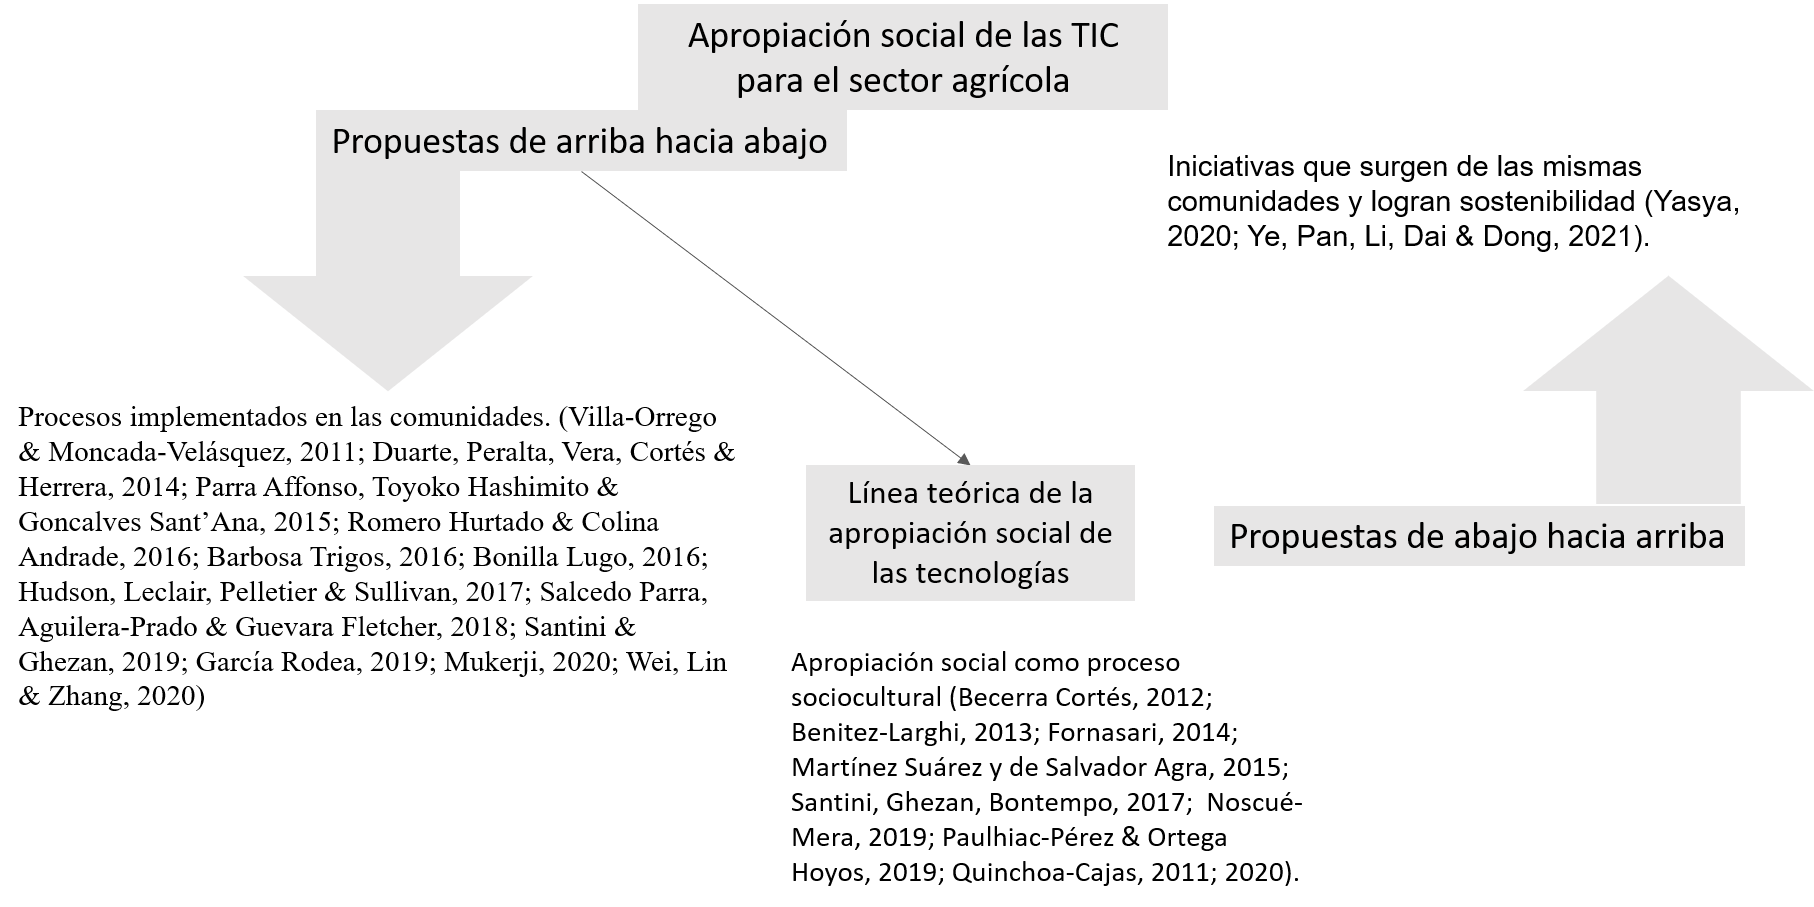
\includegraphics[width=0.85\textwidth]{fig4.png}
\caption{Apropiación social de las TIC para el sector agrícola.}
\label{fig4}
\source{Elaboración propia con base en \textcite{villa-orrego_efectos_2011,duarte_metodologipara_2014,parra_affonso_uso_2015,romero_hurtado_ensenanza_2016,barbosa_trigos_propuesta_2016,bonilla_lugo_capacitacion_2016,hudson_using_2017,salcedo_parra_compartel_2018,santini_uso_2018,garcia_rodea_uso_2019,mukerji_reexamining_2020,wei_e-commerce_2020,becerra-cortes_estudiantes_2012,benitz_laghi_lo_2013,fornasari_jovenes_2014,martinez-suarez_objetos_2015,santini_uso_2017,noscue_mera_usos_2019,paulhiac_perez_uso_2019,quinchoa-cajas_apropiacion_2011,yasya_rural_2020,ye_citizen-led_2021}.}
\end{figure}

Es común encontrar en las investigaciones citadas en este apartado que no todas se dirigen directamente a la relación de las TIC con la producción agrícola (13 de 24), sino que entienden la apropiación social como un proceso amplio que debe darse en todos los \textit{lugares} de la cotidianidad de los campesinos. Si allí se logran encontrar sus beneficios, seguramente las TIC tendrán un impacto positivo en el trabajo del sector agrícola, que hace parte también de la cotidianidad en la vida de estas familias.  

Investigaciones como la de \textcite[p. 295]{paulhiac_perez_uso_2019} cuestionan las finalidades que tienen los procesos de apropiación en estas comunidades, especialmente las que están ligadas a los procesos de desarrollo, ya que “reducen la cultura local a ideas estereotipadas. Por eso la importancia de preguntarse sobre cómo abordar la dimensión cultural con las TIC”. Los autores resaltan la importancia de ir más allá del desarrollismo y enfocar los estudios en los procesos individuales o en la subjetividad social de la apropiación. Además, los diferentes estudios abordan críticamente los acercamientos a lo agrícola desde lo productivo, basados en la eficiencia, sin tener en cuenta la gestión del conocimiento \cite{santini_uso_2017}.

La apropiación tecnológica se define “aludiendo a los procesos de interpretación y dotación de sentido implicados en las prácticas y representaciones que distintos actores construyen en torno a las Tecnologías de Información y Comunicación” \cite[p.~3]{benitz_laghi_lo_2013}. La apropiación depende de capitales culturales y simbólicos acumulados de manera individual y colectiva, “es en estos contextos y condiciones socio-culturales, con sus racionalidades y universos de sentido particulares, donde las TIC pueden volverse o no socialmente significativas y relevantes […]” \cite[p.~3]{benitz_laghi_lo_2013}.

Asimismo, uso y apropiación no van el uno sin el otro y se dan en la vida cotidiana, \textit{lugar} en el que debe estudiarse. “Una indagación por la apropiación de tecnologías debería considerar el punto de vista de los sujetos, sus prácticas, discursos y la interacción que entre ellos ocurre, mediante la cual construyen los significados y dotan de sentido su hacer” \cite[p.~5]{alvarez_cadavid_apropiacion_2011}. Los autores concluyen que son prácticas dinámicas y se dan en lo microsocial y lo macrosocial, por eso es necesario partir de los usos individuales, como también de las transformaciones cotidianas a partir de esos usos, como los temas de conversación, las formas de comunicación en sí mismas, las rutinas. 

Las investigaciones resaltan la ausencia de cobertura total de internet en las zonas rurales, así como la falta de alfabetización digital \cite{duarte_metodologipara_2014,castro_hidalgo_impacto_2014,barbosa_trigos_propuesta_2016,sanchez_davila_nuevas_2018,zapata_-_cardenas_ruralidad_2015}. En tal sentido, más que explorar la brecha digital y dar cuenta de datos estadísticos sobre el acceso, es importante trabajar lo cualitativo, sobre cómo pueden o no volverse significativas las TIC, más allá de una imposición \cite{benitz_laghi_lo_2013}. Cualquier propósito que se tenga para lograr la apropiación de las TIC debe partir de las necesidades de información y comunicación que tengan las comunidades y que estas mismas quieran para sí. No obstante, las investigaciones de abajo hacia arriba, es decir que nacen de las mismas comunidades son solamente dos en este corpus \cite{yasya_rural_2020,ye_citizen-led_2021}.

\subsection{Modelos para la apropiación social}

Las investigaciones que se presentan a continuación se enfocan conceptualmente en la apropiación social, pero su interés está en plantear modelos que puedan replicarse en diferentes comunidades agrícolas rurales. 

El primer modelo propuesto se basó en los factores que influyen en la utilización de la tecnología digital: 1. Factores personales: educación, edad, experiencia, condición física y otras condiciones psicológicas. 2. Factores sociales: normas, políticas públicas, relación con la comunidad, capital social y estructura educativa. 3. Factores del ambiente: infraestructura y condiciones geográficas \cite{savira_digitalizing_2020}. El segundo modelo se basa en la formación informal para desarrollar habilidades digitales para el emprendimiento rural \cite{ali_framework_2019}. El tercer modelo se fundamenta en: 1. Análisis de los factores que impiden el acceso y la adopción. 2. Identificación de estrategias para facilitar el acceso y la adopción. 3. Acercamientos prácticos para implementarlos \cite{matsenjwa_pro-poor_2019}.

El cuarto modelo se basa en reconocer los retos y beneficios que percibe la comunidad con el uso de las TIC, cómo se apropian y cómo el contexto permite o restringe esa apropiación \cite{hatakka_understanding_2020}. Finalmente, \textcite{acosta_nates_culturas_2014} propone tres modelos de apropiación. El primero es el de apropiación asertiva que consiste en un sentido claro y sostenido de la importancia de las TIC. El segundo modelo es el transicional, en éste solo unos pocos líderes ven la importancia de las TIC, pero no se logra establecer la relación de éstas con la vida individual y colectiva. El tercero es el inactivo en el que aún no se ha mostrado ningún interés por el uso o la apropiación de las TIC. 

\section{Discusión}

En 2010, una revisión de la literatura sobre el tema en cuestión concluyó que es necesario para el sector agrícola, entre otros aspectos: 1. el carácter participativo que deben tener las iniciativas de desarrollo para respetar las necesidades personales y grupales de la comunidad afectada; 2. aprovechar el potencial endógeno de las comunidades para evitar el fracaso de los programas; 3. incentivar y facilitar la educación en el entorno rural para su desarrollo \cite{felizzola_cruz_tecnologias_2010}. En 2017, otra revisión de la literatura indicó que los enfoques comunitarios ascendentes ofrecen algunos éxitos en el aumento de la capacidad de las comunidades \cite{roberts_review_2017}. Ahora bien, lo anterior implica reconocer que las zonas rurales necesitan estrategias diferenciales y apropiadas para la inclusión digital \cite{roberts_review_2017}. Por ejemplo, se requieren políticas públicas basadas en estudios sobre conectividad e infraestructura en el sector agrícola; como también en temas de inclusión y habilidades digitales \cite{salemink_rural_2017}.

Las reflexiones anteriores no distan mucho de lo encontrado en esta revisión de la literatura. Por un lado, la mayor parte de los estudios cuantitativos se enfocan en los usos de las TIC para la producción agrícola, mientras que, por otro lado, los estudios de apropiación social de las TIC se enfocan tanto en el sector agrícola, como en la vida cotidiana de las familias campesinas y cómo la apropiación se vuelve parte de su quehacer diario. También, por una parte, tenemos que los estudios sobre usos y adopción no presentan una mayor discusión conceptual de los términos, sino que los usan como variables de análisis, sin preocuparse por presentar sus distinciones; y, por otra parte, son los estudios latinoamericanos los que usan el término \textit{apropiación} y lo discuten teóricamente. En consecuencia, éste es un aporte relevante de esta investigación sobre apropiación social como categoría o paradigma teórico, a diferencia de los estudios previos sobre TIC y agricultura. 

\textcite[p. 18]{andres_aproximacion_2014} afirma que “en los últimos años se ha consolidado una línea de investigación referida a la apropiación social de tecnologías”. Dentro de esta línea de investigación aparece una preocupación latente y es el análisis de la apropiación social, en el auge de las tecnologías, pero también en los contextos de brecha digital. Es así como nuevas líneas aparecen, una de éstas dedicada al estudio de la apropiación social en contextos rurales y más específicamente en el sector agrícola.

Para el caso de esta revisión de la literatura se encuentran perspectivas teóricas tan diversas como los campos y disciplinas de estudio, citados más arriba. Las investigaciones que trabajan desde los usos y la adopción priorizan teorías y modelos como: Difusión de Innovaciones, la Teoría del Comportamiento Planificado, la Teoría de la Acción Razona y el modelo TAM. Otras investigaciones se enfocan en una línea denominada TIC para el desarrollo y sustentan su marco teórico alrededor de los planteamientos de Amartya Sen sobre las capacidades. Finalmente, hay una apuesta teórica, evidente en los estudios latinoamericanos, por consolidar una teoría de la apropiación social de las tecnologías, que avanza a partir de las discusiones que plantean sus autores.

A partir de lo anterior, se puede concluir que, aunque en este estudio se prioriza el enfoque en el uso y la adopción, los cuales no se distinguen conceptualmente, es la apropiación social la que adquiere mayor relevancia en cuanto a las perspectivas teóricas de las investigaciones. Ésta se entiende como la construcción de procesos sociales, en los que también la revisión de las transformaciones del contexto es parte de las iniciativas de los estudios \cite{zapata_-_cardenas_ruralidad_2015,bonilla_lugo_capacitacion_2016}.

Los usos y apropiaciones de las TIC en contextos de la brecha digital se enfocan en poblaciones en condiciones desiguales de infraestructura y de conectividad, es decir, de acceso, pero también hacen referencia a otros factores de la desigualdad social como la educación, la salud, la recreación, entre otros. Estas investigaciones permiten comprender que para lograr la apropiación social de las TIC es necesario estudiar el uso o las rutinas de uso cotidianas de los actores involucrados, porque solo allí, en su cotidianidad, es posible que las TIC hagan parte de sus representaciones socioculturales y las doten de sentido, también, para la agricultura. Por consiguiente, la apropiación social es un proceso contextualizado que requiere de una alfabetización situada y de una aproximación, principalmente, cualitativa, en la que la prioridad no es la infraestructura. Por el contrario, el dispositivo y su respectivo desarrollo tecnológico se define por las necesidades de la misma comunidad; de allí el éxito de las iniciativas de abajo hacia arriba, tan poco presentes en la literatura. 

\section{Conclusiones}

Para concretar el abordaje de las tres preguntas de investigación planteadas, se puede concluir que los enfoques de las investigaciones y las perspectivas teóricas difieren entre los estudios internacionales, africanos y asiáticos, y los estudios latinoamericanos. Los usos y la adopción son abordados, no como categorías conceptuales, sino como variables dependientes frente a diversas variables independientes. Si bien la mayoría de las investigaciones posteriores van a seguir esta misma línea, los estudios latinoamericanos son muy críticos frente a esta postura y se alejan, no solo de la teoría de Rogers de la Difusión de Innovaciones, sino también del concepto de adopción para trabajar desde el concepto de apropiación social.

Al respecto, se puede señalar que: primero, el enfoque mayoritario de las investigaciones es hacia los usos, lo cual no permite evidenciar la apropiación y, aunque estos estudios llegan a la conclusión generalizada de que hay que formar o capacitar a las comunidades, esta etapa no se desarrolla. Segundo, las investigaciones enfocadas en desarrollar habilidades digitales o capacidades en las comunidades son muy pocas, al igual que las experiencias de abajo hacia arriba. A pesar de que la literatura previa ha señalado que éste es el enfoque que tiene mayor probabilidad de éxito para el desarrollo de procesos de apropiación social, no se está investigando en esta línea.

Tercero, abordar los procesos de apropiación social para el sector agrícola implica trabajarlos desde la cotidianidad de los campesinos productores y no solamente enfocados en la productividad; las investigaciones tienden a separar ambas instancias. Esto significa que investigaciones futuras deben tener en cuenta el rol que cumple la formación en los procesos de apropiación social de las TIC. Si bien las políticas de los gobiernos se encaminan a la capacitación para el uso y la apropiación, habría que cuestionarse sobre la diferencia entre una formación y una capacitación y cómo el entendimiento mismo de la tecnología afecta la decisión que se tome sobre una o la otra, en proyectos de abajo hacia arriba. 

La última pregunta de investigación tiene que ver con lo anterior y es central para diferenciar este estudio de otros previos. Las coincidencias están en aspectos ya señalados como la importancia de priorizar la inclusión y no la conectividad; los enfoques ascendentes y participativos; y aprovechar el capital endógeno de las comunidades, que son también aportes para fortalecer esta línea de investigación y así evitar la fragmentación entre los estudios que se enfocan solo en la productividad y no en la vida cotidiana del agricultor. No obstante, esta revisión de la literatura pone en cuestión el uso de los conceptos y la manera en la que permiten o no aproximarse al fenómeno de estudio. Este es un aporte central para la consolidación del paradigma en construcción que es la apropiación de tecnologías \cite{morales_imaginacion_2017}, el cual implica un debate que va más allá de las disciplinas, pero con mayor consistencia teórica. 


\printbibliography\label{sec-bib}
% if the text is not in Portuguese, it might be necessary to use the code below instead to print the correct ABNT abbreviations [s.n.], [s.l.]
%\begin{portuguese}
%\printbibliography[title={Bibliography}]
%\end{portuguese}



\end{document}
